\documentclass[tikz, varwidth=800pt]{standalone}
\usepackage{amssymb, amsmath}

\standaloneenv{aaaa}

\begin{document}
	\begin{aaaa}
		\begin{center}	
			\fbox{%
				\begin{minipage}{0.85\linewidth}
					\centering
					\tikzset{every picture/.style={line width=0.75pt}}
					\vspace{6pt} 
					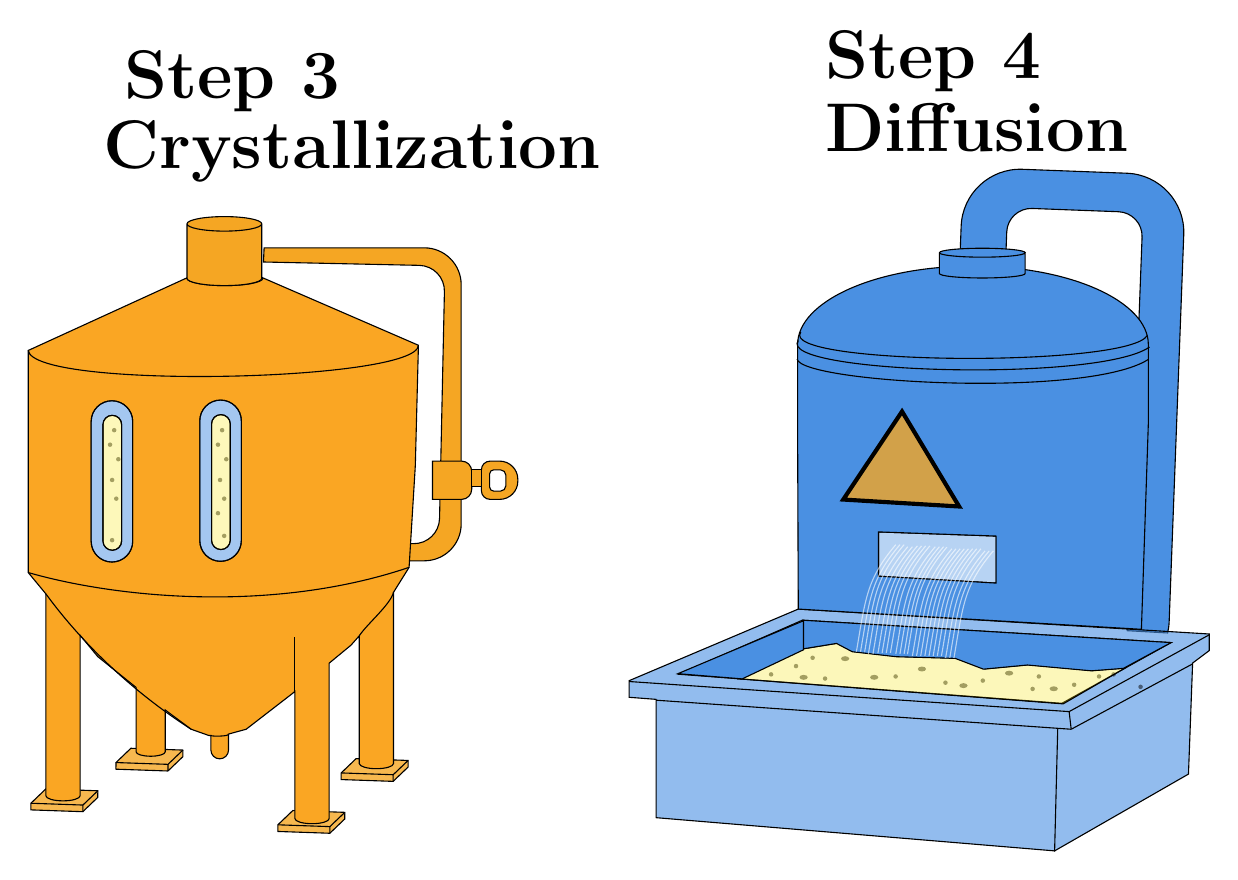
\begin{tikzpicture}[x=0.75pt,y=0.75pt,yscale=-1,xscale=1]

% ========================================
% SCHÉMA 1: Stage 3 - Crystallization (à gauche)
% ========================================
\begin{scope}[shift={(20,10)}]
    % Pas de bounding box pour Stage 3
    
	%Shape: Path Data [id:dp740170980224085] 
	\draw  [fill={rgb, 255:red, 245; green, 166; blue, 35 }  ,fill opacity=1 ] (195.8,115.8) .. controls (205.63,115.8) and (213.6,123.77) .. (213.6,133.6) -- (213.6,248.8) .. controls (213.6,258.63) and (205.63,266.6) .. (195.8,266.6) -- (188.48,266.6) -- (188.41,258.28) -- (190.54,258.33) .. controls (197.37,258.47) and (203.03,253.05) .. (203.17,246.22) -- (205.52,136.88) .. controls (205.67,130.05) and (200.25,124.39) .. (193.42,124.25) -- (118.34,122.63) -- (118.64,115.8) -- (195.8,115.8) -- cycle ;
	%Shape: Cube [id:dp5541728812371717] 
	\draw  [fill={rgb, 255:red, 245; green, 166; blue, 35 }  ,fill opacity=0.8 ] (155.78,368.79) -- (162.97,361.91) -- (188.03,362.78) -- (188,365.98) -- (180.81,372.86) -- (155.75,371.99) -- cycle ; \draw   (188.03,362.78) -- (180.84,369.66) -- (155.78,368.79) ; \draw   (180.84,369.66) -- (180.81,372.86) ;
	%Shape: Cube [id:dp17416947613627154] 
	\draw  [fill={rgb, 255:red, 245; green, 166; blue, 35 }  ,fill opacity=0.8 ] (125.28,393.79) -- (132.47,386.91) -- (157.53,387.78) -- (157.5,390.98) -- (150.31,397.86) -- (125.25,396.99) -- cycle ; \draw   (157.53,387.78) -- (150.34,394.66) -- (125.28,393.79) ; \draw   (150.34,394.66) -- (150.31,397.86) ;
	%Shape: Cube [id:dp7638862186279323] 
	\draw  [fill={rgb, 255:red, 245; green, 166; blue, 35 }  ,fill opacity=0.8 ] (47.28,363.79) -- (54.47,356.91) -- (79.53,357.78) -- (79.5,360.98) -- (72.31,367.86) -- (47.25,366.99) -- cycle ; \draw   (79.53,357.78) -- (72.34,364.66) -- (47.28,363.79) ; \draw   (72.34,364.66) -- (72.31,367.86) ;
	%Shape: Cube [id:dp4600455976097241] 
	\draw  [fill={rgb, 255:red, 245; green, 166; blue, 35 }  ,fill opacity=0.8 ] (6.28,383.4) -- (13.47,376.52) -- (38.53,377.39) -- (38.5,380.59) -- (31.31,387.47) -- (6.25,386.6) -- cycle ; \draw   (38.53,377.39) -- (31.34,384.27) -- (6.28,383.4) ; \draw   (31.34,384.27) -- (31.31,387.47) ;
	%Shape: Path Data [id:dp4984379776478407] 
	\draw  [fill={rgb, 255:red, 250; green, 166; blue, 35 }  ,fill opacity=1 ] (193,162.75) -- (191.5,220.75) -- (188.5,269.75) -- (181,281.75) -- (181,364.28) .. controls (181,365.64) and (177.31,366.75) .. (172.75,366.75) .. controls (168.19,366.75) and (164.5,365.64) .. (164.5,364.28) -- (164.5,302.73) -- (160.5,307.25) -- (150,315.91) -- (150,390.78) .. controls (150,392.14) and (146.31,393.25) .. (141.75,393.25) .. controls (137.19,393.25) and (133.5,392.14) .. (133.5,390.78) -- (133.5,329.51) -- (132,330.75) -- (110,347.75) -- (101.5,350.07) -- (101.5,357.75) .. controls (101.5,360.1) and (99.6,362) .. (97.25,362) .. controls (94.9,362) and (93,360.1) .. (93,357.75) -- (93,350.75) -- (92,350.75) -- (83.5,347.75) -- (71,338.46) -- (71,358.65) .. controls (71,359.81) and (67.87,360.75) .. (64,360.75) .. controls (60.13,360.75) and (57,359.81) .. (57,358.65) -- (57,327.62) -- (38.5,312.75) -- (30,302.47) -- (30,379.78) .. controls (30,381.14) and (26.31,382.25) .. (21.75,382.25) .. controls (17.19,382.25) and (13.5,381.14) .. (13.5,379.78) -- (13.5,282.53) -- (5,272.25) -- (5,165.25) -- (81.5,130.25) -- (81.5,130.5) .. controls (81.5,132.43) and (89.67,134) .. (99.75,134) .. controls (109.83,134) and (118,132.43) .. (118,130.5) -- (118,130.25) -- (193,162.75) -- cycle (87.67,199.17) -- (87.67,256.83) .. controls (87.67,262.36) and (92.14,266.83) .. (97.67,266.83) .. controls (103.19,266.83) and (107.67,262.36) .. (107.67,256.83) -- (107.67,199.17) .. controls (107.67,193.64) and (103.19,189.17) .. (97.67,189.17) .. controls (92.14,189.17) and (87.67,193.64) .. (87.67,199.17) -- cycle (35.33,199.5) -- (35.33,257.17) .. controls (35.33,262.69) and (39.81,267.17) .. (45.33,267.17) .. controls (50.86,267.17) and (55.33,262.69) .. (55.33,257.17) -- (55.33,199.5) .. controls (55.33,193.98) and (50.86,189.5) .. (45.33,189.5) .. controls (39.81,189.5) and (35.33,193.98) .. (35.33,199.5) -- cycle ;
	%Shape: Can [id:dp22007502420139957] 
	\draw  [fill={rgb, 255:red, 245; green, 166; blue, 35 }  ,fill opacity=1 ] (117.5,104.25) -- (117.5,130.5) .. controls (117.5,132.43) and (109.44,134) .. (99.5,134) .. controls (89.56,134) and (81.5,132.43) .. (81.5,130.5) -- (81.5,104.25) .. controls (81.5,102.32) and (89.56,100.75) .. (99.5,100.75) .. controls (109.44,100.75) and (117.5,102.32) .. (117.5,104.25) .. controls (117.5,106.18) and (109.44,107.75) .. (99.5,107.75) .. controls (89.56,107.75) and (81.5,106.18) .. (81.5,104.25) ;
	%Curve Lines [id:da4915514043760123] 
	\draw    (5,272.25) .. controls (48.5,284.75) and (123.5,291.75) .. (188.5,269.75) ;
	%Curve Lines [id:da918344478950904] 
	\draw    (5,165.25) .. controls (7.5,184.25) and (192.5,180.25) .. (193,162.75) ;
	%Curve Lines [id:da7015792738779195] 
	\draw    (13.5,282.53) .. controls (17.5,287.75) and (40,319.75) .. (83.5,347.75) ;
	%Straight Lines [id:da26177027737321357] 
	\draw    (133.5,329.51) -- (133.5,303.25) ;
	%Curve Lines [id:da2507204405100264] 
	\draw    (164.5,302.73) .. controls (168,297.25) and (179.5,287.75) .. (181,281.75) ;
	%Curve Lines [id:da9174681435393754] 
	\draw    (93,350.75) .. controls (93,351.25) and (102,351.25) .. (101.5,350.07) ;
	%Shape: Circle [id:dp242588595185817] 
	\draw  [draw opacity=0][fill={rgb, 255:red, 0; green, 0; blue, 0 }  ,fill opacity=0.5 ] (44.33,256.65) .. controls (44.33,256.05) and (44.82,255.57) .. (45.42,255.57) .. controls (46.01,255.57) and (46.5,256.05) .. (46.5,256.65) .. controls (46.5,257.25) and (46.01,257.73) .. (45.42,257.73) .. controls (44.82,257.73) and (44.33,257.25) .. (44.33,256.65) -- cycle ;
	%Shape: Circle [id:dp23321530676438273] 
	\draw  [draw opacity=0][fill={rgb, 255:red, 0; green, 0; blue, 0 }  ,fill opacity=0.5 ] (46.33,236.65) .. controls (46.33,236.05) and (46.82,235.57) .. (47.42,235.57) .. controls (48.01,235.57) and (48.5,236.05) .. (48.5,236.65) .. controls (48.5,237.25) and (48.01,237.73) .. (47.42,237.73) .. controls (46.82,237.73) and (46.33,237.25) .. (46.33,236.65) -- cycle ;
	%Shape: Circle [id:dp5098212117846179] 
	\draw  [draw opacity=0][fill={rgb, 255:red, 0; green, 0; blue, 0 }  ,fill opacity=0.5 ] (44.33,227.65) .. controls (44.33,227.05) and (44.82,226.57) .. (45.42,226.57) .. controls (46.01,226.57) and (46.5,227.05) .. (46.5,227.65) .. controls (46.5,228.25) and (46.01,228.73) .. (45.42,228.73) .. controls (44.82,228.73) and (44.33,228.25) .. (44.33,227.65) -- cycle ;
	%Shape: Circle [id:dp36591736603179903] 
	\draw  [draw opacity=0][fill={rgb, 255:red, 0; green, 0; blue, 0 }  ,fill opacity=0.5 ] (47.33,217.65) .. controls (47.33,217.05) and (47.82,216.57) .. (48.42,216.57) .. controls (49.01,216.57) and (49.5,217.05) .. (49.5,217.65) .. controls (49.5,218.25) and (49.01,218.73) .. (48.42,218.73) .. controls (47.82,218.73) and (47.33,218.25) .. (47.33,217.65) -- cycle ;
	%Shape: Circle [id:dp9578926552919954] 
	\draw  [draw opacity=0][fill={rgb, 255:red, 0; green, 0; blue, 0 }  ,fill opacity=0.5 ] (43.33,210.65) .. controls (43.33,210.05) and (43.82,209.57) .. (44.42,209.57) .. controls (45.01,209.57) and (45.5,210.05) .. (45.5,210.65) .. controls (45.5,211.25) and (45.01,211.73) .. (44.42,211.73) .. controls (43.82,211.73) and (43.33,211.25) .. (43.33,210.65) -- cycle ;
	%Shape: Circle [id:dp6180370300786379] 
	\draw  [draw opacity=0][fill={rgb, 255:red, 0; green, 0; blue, 0 }  ,fill opacity=0.5 ] (45.33,203.65) .. controls (45.33,203.05) and (45.82,202.57) .. (46.42,202.57) .. controls (47.01,202.57) and (47.5,203.05) .. (47.5,203.65) .. controls (47.5,204.25) and (47.01,204.73) .. (46.42,204.73) .. controls (45.82,204.73) and (45.33,204.25) .. (45.33,203.65) -- cycle ;
	%Shape: Circle [id:dp4494799289937478] 
	\draw  [draw opacity=0][fill={rgb, 255:red, 0; green, 0; blue, 0 }  ,fill opacity=0.5 ] (98.33,254.58) .. controls (98.33,253.99) and (98.82,253.5) .. (99.42,253.5) .. controls (100.01,253.5) and (100.5,253.99) .. (100.5,254.58) .. controls (100.5,255.18) and (100.01,255.67) .. (99.42,255.67) .. controls (98.82,255.67) and (98.33,255.18) .. (98.33,254.58) -- cycle ;
	%Shape: Circle [id:dp4825326058906537] 
	\draw  [draw opacity=0][fill={rgb, 255:red, 0; green, 0; blue, 0 }  ,fill opacity=0.5 ] (95.33,243.65) .. controls (95.33,243.05) and (95.82,242.57) .. (96.42,242.57) .. controls (97.01,242.57) and (97.5,243.05) .. (97.5,243.65) .. controls (97.5,244.25) and (97.01,244.73) .. (96.42,244.73) .. controls (95.82,244.73) and (95.33,244.25) .. (95.33,243.65) -- cycle ;
	%Shape: Circle [id:dp7252624860204063] 
	\draw  [draw opacity=0][fill={rgb, 255:red, 0; green, 0; blue, 0 }  ,fill opacity=0.5 ] (98.33,236.65) .. controls (98.33,236.05) and (98.82,235.57) .. (99.42,235.57) .. controls (100.01,235.57) and (100.5,236.05) .. (100.5,236.65) .. controls (100.5,237.25) and (100.01,237.73) .. (99.42,237.73) .. controls (98.82,237.73) and (98.33,237.25) .. (98.33,236.65) -- cycle ;
	%Shape: Circle [id:dp84434403201706] 
	\draw  [draw opacity=0][fill={rgb, 255:red, 0; green, 0; blue, 0 }  ,fill opacity=0.5 ] (96.33,227.65) .. controls (96.33,227.05) and (96.82,226.57) .. (97.42,226.57) .. controls (98.01,226.57) and (98.5,227.05) .. (98.5,227.65) .. controls (98.5,228.25) and (98.01,228.73) .. (97.42,228.73) .. controls (96.82,228.73) and (96.33,228.25) .. (96.33,227.65) -- cycle ;
	%Shape: Circle [id:dp8640128060431128] 
	\draw  [draw opacity=0][fill={rgb, 255:red, 0; green, 0; blue, 0 }  ,fill opacity=0.5 ] (99.33,217.65) .. controls (99.33,217.05) and (99.82,216.57) .. (100.42,216.57) .. controls (101.01,216.57) and (101.5,217.05) .. (101.5,217.65) .. controls (101.5,218.25) and (101.01,218.73) .. (100.42,218.73) .. controls (99.82,218.73) and (99.33,218.25) .. (99.33,217.65) -- cycle ;
	%Shape: Circle [id:dp528873265919408] 
	\draw  [draw opacity=0][fill={rgb, 255:red, 0; green, 0; blue, 0 }  ,fill opacity=0.5 ] (95.33,210.65) .. controls (95.33,210.05) and (95.82,209.57) .. (96.42,209.57) .. controls (97.01,209.57) and (97.5,210.05) .. (97.5,210.65) .. controls (97.5,211.25) and (97.01,211.73) .. (96.42,211.73) .. controls (95.82,211.73) and (95.33,211.25) .. (95.33,210.65) -- cycle ;
	%Shape: Circle [id:dp07387891813843273] 
	\draw  [draw opacity=0][fill={rgb, 255:red, 0; green, 0; blue, 0 }  ,fill opacity=0.5 ] (97.33,203.65) .. controls (97.33,203.05) and (97.82,202.57) .. (98.42,202.57) .. controls (99.01,202.57) and (99.5,203.05) .. (99.5,203.65) .. controls (99.5,204.25) and (99.01,204.73) .. (98.42,204.73) .. controls (97.82,204.73) and (97.33,204.25) .. (97.33,203.65) -- cycle ;
	%Rounded Same Side Corner Rect [id:dp9287106514136438] 
	\draw  [fill={rgb, 255:red, 245; green, 166; blue, 35 }  ,fill opacity=1 ] (213.78,218.56) .. controls (216.48,218.56) and (218.67,220.74) .. (218.67,223.44) -- (218.67,232.11) .. controls (218.67,234.81) and (216.48,237) .. (213.78,237) -- (199.78,237) .. controls (199.78,237) and (199.78,237) .. (199.78,237) -- (199.78,218.56) .. controls (199.78,218.56) and (199.78,218.56) .. (199.78,218.56) -- cycle ;
	%Shape: Path Data [id:dp6073502102682435] 
	\draw  [fill={rgb, 255:red, 245; green, 166; blue, 35 }  ,fill opacity=1 ] (240.89,227.33) -- (240.89,228.22) .. controls (240.89,233.07) and (236.96,237) .. (232.11,237) -- (227.56,237) .. controls (225.23,237) and (223.33,235.11) .. (223.33,232.77) -- (223.33,222.79) .. controls (223.33,220.45) and (225.23,218.56) .. (227.56,218.56) -- (232.11,218.56) .. controls (236.96,218.56) and (240.89,222.49) .. (240.89,227.33) -- cycle (232.57,222.78) -- (229.21,222.78) .. controls (228.17,222.78) and (227.33,223.62) .. (227.33,224.65) -- (227.33,231.13) .. controls (227.33,232.16) and (228.17,233) .. (229.21,233) -- (232.57,233) .. controls (233.98,233) and (235.11,231.86) .. (235.11,230.46) -- (235.11,225.31) .. controls (235.11,223.91) and (233.98,222.78) .. (232.57,222.78) -- cycle ;
	%Shape: Rectangle [id:dp1777709869535974] 
	\draw  [fill={rgb, 255:red, 245; green, 166; blue, 35 }  ,fill opacity=1 ] (218.67,222.79) -- (223.33,222.79) -- (223.33,230.78) -- (218.67,230.78) -- cycle ;
	%Shape: Path Data [id:dp8659172700956831] 
	\draw  [fill={rgb, 255:red, 74; green, 144; blue, 226 }  ,fill opacity=0.5 ] (97.67,189.17) .. controls (103.19,189.17) and (107.67,193.64) .. (107.67,199.17) -- (107.67,256.83) .. controls (107.67,262.36) and (103.19,266.83) .. (97.67,266.83) .. controls (92.14,266.83) and (87.67,262.36) .. (87.67,256.83) -- (87.67,199.17) .. controls (87.67,193.64) and (92.14,189.17) .. (97.67,189.17) -- cycle (93.33,200.67) -- (93.33,256.67) .. controls (93.33,259.15) and (95.35,261.17) .. (97.83,261.17) .. controls (100.32,261.17) and (102.33,259.15) .. (102.33,256.67) -- (102.33,200.67) .. controls (102.33,198.18) and (100.32,196.17) .. (97.83,196.17) .. controls (95.35,196.17) and (93.33,198.18) .. (93.33,200.67) -- cycle ;
	%Shape: Path Data [id:dp42692768176603757] 
	\draw  [fill={rgb, 255:red, 248; green, 231; blue, 28 }  ,fill opacity=0.3 ] (97.83,196.17) .. controls (100.32,196.17) and (102.33,198.18) .. (102.33,200.67) -- (102.33,256.67) .. controls (102.33,259.15) and (100.32,261.17) .. (97.83,261.17) .. controls (95.35,261.17) and (93.33,259.15) .. (93.33,256.67) -- (93.33,200.67) .. controls (93.33,198.18) and (95.35,196.17) .. (97.83,196.17) -- cycle ;
	%Shape: Path Data [id:dp33523580686470944] 
	\draw  [fill={rgb, 255:red, 74; green, 144; blue, 226 }  ,fill opacity=0.5 ] (45.33,189.5) .. controls (50.86,189.5) and (55.33,193.98) .. (55.33,199.5) -- (55.33,257.17) .. controls (55.33,262.69) and (50.86,267.17) .. (45.33,267.17) .. controls (39.81,267.17) and (35.33,262.69) .. (35.33,257.17) -- (35.33,199.5) .. controls (35.33,193.98) and (39.81,189.5) .. (45.33,189.5) -- cycle (41,201) -- (41,257) .. controls (41,259.49) and (43.01,261.5) .. (45.5,261.5) .. controls (47.99,261.5) and (50,259.49) .. (50,257) -- (50,201) .. controls (50,198.51) and (47.99,196.5) .. (45.5,196.5) .. controls (43.01,196.5) and (41,198.51) .. (41,201) -- cycle ;
	%Shape: Path Data [id:dp8349830493783591] 
	\draw  [fill={rgb, 255:red, 248; green, 231; blue, 28 }  ,fill opacity=0.3 ] (45.5,196.5) .. controls (47.99,196.5) and (50,198.51) .. (50,201) -- (50,257) .. controls (50,259.49) and (47.99,261.5) .. (45.5,261.5) .. controls (43.01,261.5) and (41,259.49) .. (41,257) -- (41,201) .. controls (41,198.51) and (43.01,196.5) .. (45.5,196.5) -- cycle ;

	% Text Node
	\draw (40,53.4) node [anchor=north west][inner sep=0.75pt]  [font=\Huge] [align=left] {\textbf{Crystallization}};

	% Text Node
	\draw (50,20) node [anchor=north west][inner sep=0.75pt]  [font=\Huge] [align=left] {\textbf{Step 3}};

\end{scope}

% ========================================
% SCHÉMA 2: Step 4 - Diffusion (à droite)
% ========================================
\begin{scope}[shift={(300,10)}]
    % Bounding box interne pour Step 4 (commentée)
    % \draw (0,0) rectangle (610,440);
    
	%Shape: Polygon [id:ds4064514405975208] 
	\draw  [fill={rgb, 255:red, 74; green, 144; blue, 226 }  ,fill opacity=0.4 ] (191.33,277.33) -- (134.67,274) -- (134.67,252.67) -- (191.33,254.67) -- cycle ;
	%Shape: Path Data [id:dp35119156762297865] 
	\draw  [fill={rgb, 255:red, 74; green, 144; blue, 226 }  ,fill opacity=1 ] (204.01,77.96) -- (254.35,79.86) .. controls (270.06,80.45) and (282.33,93.68) .. (281.73,109.39) -- (274.7,295.83) .. controls (274.63,297.73) and (274.37,299.58) .. (273.95,301.36) -- (254.49,300.26) -- (261.64,110.64) .. controls (261.89,104.13) and (256.81,98.66) .. (250.3,98.41) -- (208.67,96.84) .. controls (202.16,96.6) and (196.68,101.67) .. (196.44,108.18) -- (195.43,134.86) -- (173.39,134.22) -- (174.48,105.35) .. controls (175.07,89.63) and (188.29,77.37) .. (204.01,77.96) -- cycle ;
	%Shape: Polygon [id:ds8510150227056082] 
	\draw  [fill={rgb, 255:red, 74; green, 144; blue, 226 }  ,fill opacity=0.6 ] (284,369.35) -- (219.5,406.35) -- (27.5,390.35) -- (27.5,333.35) -- (14.5,332.35) -- (14.5,324.35) -- (96,289.85) -- (294,301.85) -- (294,309.85) -- (286,315.85) -- cycle ;
	%Straight Lines [id:da3654938941022118] 
	\draw    (27.5,333.75) -- (227.5,347.75) ;
	%Straight Lines [id:da12503765856262283] 
	\draw    (227.5,347.75) -- (286,316.25) ;
	%Straight Lines [id:da5166787893395551] 
	\draw    (14.5,324.75) -- (226.5,339.25) ;
	%Straight Lines [id:da9333334976241038] 
	\draw    (226.5,339.25) -- (294,302.25) ;
	%Straight Lines [id:da998347705627445] 
	\draw    (226.5,339.25) -- (227.5,347.75) ;
	%Straight Lines [id:da6909125343637312] 
	\draw [fill={rgb, 255:red, 74; green, 144; blue, 226 }  ,fill opacity=1 ]   (219.5,406.75) -- (221,347.75) ;
	%Shape: Path Data [id:dp22686871453193025] 
	\draw  [fill={rgb, 255:red, 74; green, 144; blue, 226 }  ,fill opacity=1 ] (95.67,162.43) .. controls (95.67,141.54) and (133.5,124.6) .. (180.17,124.6) .. controls (226.83,124.6) and (264.67,141.54) .. (264.67,162.43) -- (264.67,200.27) -- (261.33,299.6) -- (96,289.85) -- (95.67,200.27) -- (95.67,162.43) -- cycle (191.33,277.33) -- (191.33,254.67) -- (134.67,252.67) -- (134.67,274) -- (191.33,277.33) -- cycle ;
	%Shape: Polygon [id:ds6961869257044322] 
	\draw  [fill={rgb, 255:red, 245; green, 166; blue, 35 }  ,fill opacity=0.8 ][line width=1.5]  (146,194.67) -- (173.5,240.42) -- (117.67,237.08) -- cycle ;
	%Curve Lines [id:da6943308282030407] 
	\draw    (95.4,169.4) .. controls (98,181) and (235.2,188.4) .. (264.6,169.6) ;
	%Curve Lines [id:da6433057190127286] 
	\draw    (96,160.4) .. controls (84.6,176.4) and (240.8,180.8) .. (265.2,163.6) ;
	%Curve Lines [id:da9012210298300685] 
	\draw    (97.2,156.4) .. controls (85.8,172.4) and (255.2,173.6) .. (264.2,158) ;
	%Shape: Polygon [id:ds37127469012501024] 
	\draw   (223,335.25) -- (66.8,323.2) -- (97.2,308.8) -- (114.4,306) -- (122,310) -- (143.2,312.4) -- (171.6,313.2) -- (185.2,318.4) -- (206.4,316.4) -- (237.2,319.2) -- (252.8,318) -- cycle ;
	%Shape: Polygon [id:ds5590572248497979] 
	\draw  [fill={rgb, 255:red, 255; green, 255; blue, 255 }  ,fill opacity=1 ] (223,335.25) -- (38.5,321.25) -- (98,295.2) -- (275.6,306) -- cycle ;
	%Shape: Circle [id:dp39275733445484073] 
	\draw  [draw opacity=0][fill={rgb, 255:red, 0; green, 0; blue, 0 }  ,fill opacity=0.5 ] (81.83,321.32) .. controls (81.83,320.72) and (82.32,320.23) .. (82.92,320.23) .. controls (83.51,320.23) and (84,320.72) .. (84,321.32) .. controls (84,321.92) and (83.51,322.4) .. (82.92,322.4) .. controls (82.32,322.4) and (81.83,321.92) .. (81.83,321.32) -- cycle ;
	%Shape: Ellipse [id:dp31448593349952836] 
	\draw  [draw opacity=0][fill={rgb, 255:red, 0; green, 0; blue, 0 }  ,fill opacity=0.5 ] (96.58,322.73) .. controls (96.58,322.07) and (97.48,321.54) .. (98.58,321.54) .. controls (99.69,321.54) and (100.58,322.07) .. (100.58,322.73) .. controls (100.58,323.39) and (99.69,323.92) .. (98.58,323.92) .. controls (97.48,323.92) and (96.58,323.39) .. (96.58,322.73) -- cycle ;
	%Shape: Ellipse [id:dp35150330418693454] 
	\draw  [draw opacity=0][fill={rgb, 255:red, 0; green, 0; blue, 0 }  ,fill opacity=0.5 ] (217.08,328.23) .. controls (217.08,327.57) and (217.98,327.04) .. (219.08,327.04) .. controls (220.19,327.04) and (221.08,327.57) .. (221.08,328.23) .. controls (221.08,328.89) and (220.19,329.42) .. (219.08,329.42) .. controls (217.98,329.42) and (217.08,328.89) .. (217.08,328.23) -- cycle ;
	%Shape: Ellipse [id:dp49355274026905915] 
	\draw  [draw opacity=0][fill={rgb, 255:red, 0; green, 0; blue, 0 }  ,fill opacity=0.5 ] (116.58,313.73) .. controls (116.58,313.07) and (117.48,312.54) .. (118.58,312.54) .. controls (119.69,312.54) and (120.58,313.07) .. (120.58,313.73) .. controls (120.58,314.39) and (119.69,314.92) .. (118.58,314.92) .. controls (117.48,314.92) and (116.58,314.39) .. (116.58,313.73) -- cycle ;
	%Shape: Ellipse [id:dp24462867957943346] 
	\draw  [draw opacity=0][fill={rgb, 255:red, 0; green, 0; blue, 0 }  ,fill opacity=0.5 ] (130.58,322.73) .. controls (130.58,322.07) and (131.48,321.54) .. (132.58,321.54) .. controls (133.69,321.54) and (134.58,322.07) .. (134.58,322.73) .. controls (134.58,323.39) and (133.69,323.92) .. (132.58,323.92) .. controls (131.48,323.92) and (130.58,323.39) .. (130.58,322.73) -- cycle ;
	%Shape: Ellipse [id:dp37076534245874304] 
	\draw  [draw opacity=0][fill={rgb, 255:red, 0; green, 0; blue, 0 }  ,fill opacity=0.5 ] (153.58,318.73) .. controls (153.58,318.07) and (154.48,317.54) .. (155.58,317.54) .. controls (156.69,317.54) and (157.58,318.07) .. (157.58,318.73) .. controls (157.58,319.39) and (156.69,319.92) .. (155.58,319.92) .. controls (154.48,319.92) and (153.58,319.39) .. (153.58,318.73) -- cycle ;
	%Shape: Ellipse [id:dp0958160725182382] 
	\draw  [draw opacity=0][fill={rgb, 255:red, 0; green, 0; blue, 0 }  ,fill opacity=0.5 ] (173.58,326.73) .. controls (173.58,326.07) and (174.48,325.54) .. (175.58,325.54) .. controls (176.69,325.54) and (177.58,326.07) .. (177.58,326.73) .. controls (177.58,327.39) and (176.69,327.92) .. (175.58,327.92) .. controls (174.48,327.92) and (173.58,327.39) .. (173.58,326.73) -- cycle ;
	%Shape: Ellipse [id:dp346353664426017] 
	\draw  [draw opacity=0][fill={rgb, 255:red, 0; green, 0; blue, 0 }  ,fill opacity=0.5 ] (195.58,320.73) .. controls (195.58,320.07) and (196.48,319.54) .. (197.58,319.54) .. controls (198.69,319.54) and (199.58,320.07) .. (199.58,320.73) .. controls (199.58,321.39) and (198.69,321.92) .. (197.58,321.92) .. controls (196.48,321.92) and (195.58,321.39) .. (195.58,320.73) -- cycle ;
	%Shape: Circle [id:dp10529033599899029] 
	\draw  [draw opacity=0][fill={rgb, 255:red, 0; green, 0; blue, 0 }  ,fill opacity=0.5 ] (101.83,313.32) .. controls (101.83,312.72) and (102.32,312.23) .. (102.92,312.23) .. controls (103.51,312.23) and (104,312.72) .. (104,313.32) .. controls (104,313.92) and (103.51,314.4) .. (102.92,314.4) .. controls (102.32,314.4) and (101.83,313.92) .. (101.83,313.32) -- cycle ;
	%Shape: Circle [id:dp6006715128229848] 
	\draw  [draw opacity=0][fill={rgb, 255:red, 0; green, 0; blue, 0 }  ,fill opacity=0.5 ] (93.83,317.32) .. controls (93.83,316.72) and (94.32,316.23) .. (94.92,316.23) .. controls (95.51,316.23) and (96,316.72) .. (96,317.32) .. controls (96,317.92) and (95.51,318.4) .. (94.92,318.4) .. controls (94.32,318.4) and (93.83,317.92) .. (93.83,317.32) -- cycle ;
	%Shape: Circle [id:dp8376114765926564] 
	\draw  [draw opacity=0][fill={rgb, 255:red, 0; green, 0; blue, 0 }  ,fill opacity=0.5 ] (107.83,323.32) .. controls (107.83,322.72) and (108.32,322.23) .. (108.92,322.23) .. controls (109.51,322.23) and (110,322.72) .. (110,323.32) .. controls (110,323.92) and (109.51,324.4) .. (108.92,324.4) .. controls (108.32,324.4) and (107.83,323.92) .. (107.83,323.32) -- cycle ;
	%Shape: Circle [id:dp9333892738956396] 
	\draw  [draw opacity=0][fill={rgb, 255:red, 0; green, 0; blue, 0 }  ,fill opacity=0.5 ] (141.83,322.32) .. controls (141.83,321.72) and (142.32,321.23) .. (142.92,321.23) .. controls (143.51,321.23) and (144,321.72) .. (144,322.32) .. controls (144,322.92) and (143.51,323.4) .. (142.92,323.4) .. controls (142.32,323.4) and (141.83,322.92) .. (141.83,322.32) -- cycle ;
	%Shape: Circle [id:dp41782673093606466] 
	\draw  [draw opacity=0][fill={rgb, 255:red, 0; green, 0; blue, 0 }  ,fill opacity=0.5 ] (165.83,325.32) .. controls (165.83,324.72) and (166.32,324.23) .. (166.92,324.23) .. controls (167.51,324.23) and (168,324.72) .. (168,325.32) .. controls (168,325.92) and (167.51,326.4) .. (166.92,326.4) .. controls (166.32,326.4) and (165.83,325.92) .. (165.83,325.32) -- cycle ;
	%Shape: Circle [id:dp8004691899867343] 
	\draw  [draw opacity=0][fill={rgb, 255:red, 0; green, 0; blue, 0 }  ,fill opacity=0.5 ] (183.83,324.32) .. controls (183.83,323.72) and (184.32,323.23) .. (184.92,323.23) .. controls (185.51,323.23) and (186,323.72) .. (186,324.32) .. controls (186,324.92) and (185.51,325.4) .. (184.92,325.4) .. controls (184.32,325.4) and (183.83,324.92) .. (183.83,324.32) -- cycle ;
	%Shape: Circle [id:dp25926736046598694] 
	\draw  [draw opacity=0][fill={rgb, 255:red, 0; green, 0; blue, 0 }  ,fill opacity=0.5 ] (207.83,328.32) .. controls (207.83,327.72) and (208.32,327.23) .. (208.92,327.23) .. controls (209.51,327.23) and (210,327.72) .. (210,328.32) .. controls (210,328.92) and (209.51,329.4) .. (208.92,329.4) .. controls (208.32,329.4) and (207.83,328.92) .. (207.83,328.32) -- cycle ;
	%Shape: Circle [id:dp5949054636991938] 
	\draw  [draw opacity=0][fill={rgb, 255:red, 0; green, 0; blue, 0 }  ,fill opacity=0.5 ] (227.83,326.32) .. controls (227.83,325.72) and (228.32,325.23) .. (228.92,325.23) .. controls (229.51,325.23) and (230,325.72) .. (230,326.32) .. controls (230,326.92) and (229.51,327.4) .. (228.92,327.4) .. controls (228.32,327.4) and (227.83,326.92) .. (227.83,326.32) -- cycle ;
	%Shape: Circle [id:dp7654963881788195] 
	\draw  [draw opacity=0][fill={rgb, 255:red, 0; green, 0; blue, 0 }  ,fill opacity=0.5 ] (246.83,321.32) .. controls (246.83,320.72) and (247.32,320.23) .. (247.92,320.23) .. controls (248.51,320.23) and (249,320.72) .. (249,321.32) .. controls (249,321.92) and (248.51,322.4) .. (247.92,322.4) .. controls (247.32,322.4) and (246.83,321.92) .. (246.83,321.32) -- cycle ;
	%Shape: Circle [id:dp21098468732819518] 
	\draw  [draw opacity=0][fill={rgb, 255:red, 0; green, 0; blue, 0 }  ,fill opacity=0.5 ] (259.83,327.32) .. controls (259.83,326.72) and (260.32,326.23) .. (260.92,326.23) .. controls (261.51,326.23) and (262,326.72) .. (262,327.32) .. controls (262,327.92) and (261.51,328.4) .. (260.92,328.4) .. controls (260.32,328.4) and (259.83,327.92) .. (259.83,327.32) -- cycle ;
	%Shape: Circle [id:dp8619916951698095] 
	\draw  [draw opacity=0][fill={rgb, 255:red, 0; green, 0; blue, 0 }  ,fill opacity=0.5 ] (239.83,322.32) .. controls (239.83,321.72) and (240.32,321.23) .. (240.92,321.23) .. controls (241.51,321.23) and (242,321.72) .. (242,322.32) .. controls (242,322.92) and (241.51,323.4) .. (240.92,323.4) .. controls (240.32,323.4) and (239.83,322.92) .. (239.83,322.32) -- cycle ;
	%Shape: Circle [id:dp04074607388341378] 
	\draw  [draw opacity=0][fill={rgb, 255:red, 0; green, 0; blue, 0 }  ,fill opacity=0.5 ] (210.83,322.32) .. controls (210.83,321.72) and (211.32,321.23) .. (211.92,321.23) .. controls (212.51,321.23) and (213,321.72) .. (213,322.32) .. controls (213,322.92) and (212.51,323.4) .. (211.92,323.4) .. controls (211.32,323.4) and (210.83,322.92) .. (210.83,322.32) -- cycle ;
	%Shape: Polygon [id:ds7403641988997934] 
	\draw  [fill={rgb, 255:red, 248; green, 231; blue, 28 }  ,fill opacity=0.3 ] (223.63,335.52) -- (67.43,323.47) -- (97.83,309.07) -- (115.03,306.27) -- (122.63,310.27) -- (143.83,312.67) -- (172.23,313.47) -- (185.83,318.67) -- (207.03,316.67) -- (237.83,319.47) -- (253.43,318.27) -- cycle ;
	
	%Shape: Path Data [id:dp15167970180235957] 
	\draw  [fill={rgb, 255:red, 74; green, 144; blue, 226 }  ,fill opacity=1 ] (98,295.2) -- (275.6,306) -- (252.68,318.41) -- (237.2,319.6) -- (206.4,316.8) -- (185.2,318.8) -- (171.6,313.6) -- (143.2,312.8) -- (122,310.4) -- (114.4,306.4) -- (97.33,309.18) -- (98,295.2) -- cycle ;
	%Shape: Can [id:dp5313849140147021] 
	\draw  [fill={rgb, 255:red, 74; green, 144; blue, 226 }  ,fill opacity=1 ] (205.33,118.15) -- (205.33,128.18) .. controls (205.33,129.37) and (196.08,130.33) .. (184.67,130.33) .. controls (173.25,130.33) and (164,129.37) .. (164,128.18) -- (164,118.15) .. controls (164,116.96) and (173.25,116) .. (184.67,116) .. controls (196.08,116) and (205.33,116.96) .. (205.33,118.15) .. controls (205.33,119.34) and (196.08,120.3) .. (184.67,120.3) .. controls (173.25,120.3) and (164,119.34) .. (164,118.15) ;
	%Curve Lines [id:da11890683366170429] 
	\draw [color={rgb, 255:red, 255; green, 255; blue, 255 }  ,draw opacity=0.6 ]   (143,258.8) .. controls (128.8,275.6) and (128.4,284.8) .. (124,310.4) ;
	%Curve Lines [id:da6407453953597059] 
	\draw [color={rgb, 255:red, 255; green, 255; blue, 255 }  ,draw opacity=0.6 ]   (145,258.8) .. controls (130.8,275.6) and (130.4,284.8) .. (126,310.4) ;
	%Curve Lines [id:da16506423302123296] 
	\draw [color={rgb, 255:red, 255; green, 255; blue, 255 }  ,draw opacity=0.6 ]   (147,258.8) .. controls (132.8,275.6) and (132.4,284.8) .. (128,310.4) ;
	%Curve Lines [id:da9514382268865446] 
	\draw [color={rgb, 255:red, 255; green, 255; blue, 255 }  ,draw opacity=0.6 ]   (148.78,259.8) .. controls (134.58,276.6) and (134.18,285.8) .. (129.78,311.4) ;
	%Curve Lines [id:da2567602694986312] 
	\draw [color={rgb, 255:red, 255; green, 255; blue, 255 }  ,draw opacity=0.6 ]   (151,259.8) .. controls (136.8,276.6) and (136.4,285.8) .. (132,311.4) ;
	%Curve Lines [id:da05920584738558232] 
	\draw [color={rgb, 255:red, 255; green, 255; blue, 255 }  ,draw opacity=0.6 ]   (153.4,259.4) .. controls (139.2,276.2) and (138.8,285.4) .. (134.4,311) ;
	%Curve Lines [id:da2900942609843956] 
	\draw [color={rgb, 255:red, 255; green, 255; blue, 255 }  ,draw opacity=0.6 ]   (155.4,259.4) .. controls (141.2,276.2) and (140.8,285.4) .. (136.4,311) ;
	%Curve Lines [id:da23451953818375448] 
	\draw [color={rgb, 255:red, 255; green, 255; blue, 255 }  ,draw opacity=0.6 ]   (157.4,259.4) .. controls (143.2,276.2) and (142.8,285.4) .. (138.4,311) ;
	%Curve Lines [id:da5811681610315563] 
	\draw [color={rgb, 255:red, 255; green, 255; blue, 255 }  ,draw opacity=0.6 ]   (159.4,259.4) .. controls (145.2,276.2) and (144.8,285.4) .. (140.4,311) ;
	%Curve Lines [id:da9402256005421262] 
	\draw [color={rgb, 255:red, 255; green, 255; blue, 255 }  ,draw opacity=0.6 ]   (162,259.8) .. controls (147.8,276.6) and (147.4,285.8) .. (143,311.4) ;
	%Curve Lines [id:da5764797473447335] 
	\draw [color={rgb, 255:red, 255; green, 255; blue, 255 }  ,draw opacity=0.6 ]   (164,259.8) .. controls (149.8,276.6) and (149.4,285.8) .. (145,311.4) ;
	%Curve Lines [id:da38140809653388486] 
	\draw [color={rgb, 255:red, 255; green, 255; blue, 255 }  ,draw opacity=0.6 ]   (166,259.8) .. controls (151.8,276.6) and (151.4,285.8) .. (147,311.4) ;
	%Curve Lines [id:da7302677970246141] 
	\draw [color={rgb, 255:red, 255; green, 255; blue, 255 }  ,draw opacity=0.6 ]   (167.6,260) .. controls (153.4,276.8) and (153,286) .. (148.6,311.6) ;
	%Curve Lines [id:da26833662389498014] 
	\draw [color={rgb, 255:red, 255; green, 255; blue, 255 }  ,draw opacity=0.6 ]   (170,260.8) .. controls (155.8,277.6) and (155.4,286.8) .. (151,312.4) ;
	%Curve Lines [id:da8034948507944907] 
	\draw [color={rgb, 255:red, 255; green, 255; blue, 255 }  ,draw opacity=0.6 ]   (172,260.8) .. controls (157.8,277.6) and (157.4,286.8) .. (153,312.4) ;
	%Curve Lines [id:da6322672557369288] 
	\draw [color={rgb, 255:red, 255; green, 255; blue, 255 }  ,draw opacity=0.6 ]   (174,260.8) .. controls (159.8,277.6) and (159.4,286.8) .. (155,312.4) ;
	%Curve Lines [id:da6446209891733293] 
	\draw [color={rgb, 255:red, 255; green, 255; blue, 255 }  ,draw opacity=0.6 ]   (176,260.8) .. controls (161.8,277.6) and (161.4,286.8) .. (157,312.4) ;
	%Curve Lines [id:da033700031234834116] 
	\draw [color={rgb, 255:red, 255; green, 255; blue, 255 }  ,draw opacity=0.6 ]   (178,260.8) .. controls (163.8,277.6) and (163.4,286.8) .. (159,312.4) ;
	%Curve Lines [id:da49289972726629216] 
	\draw [color={rgb, 255:red, 255; green, 255; blue, 255 }  ,draw opacity=0.6 ]   (180,260.8) .. controls (165.8,277.6) and (165.4,286.8) .. (161,312.4) ;
	%Curve Lines [id:da025876931878601073] 
	\draw [color={rgb, 255:red, 255; green, 255; blue, 255 }  ,draw opacity=0.6 ]   (182,260.8) .. controls (167.8,277.6) and (167.4,286.8) .. (163,312.4) ;
	%Curve Lines [id:da37977946993571066] 
	\draw [color={rgb, 255:red, 255; green, 255; blue, 255 }  ,draw opacity=0.6 ]   (184,260.8) .. controls (169.8,277.6) and (169.4,286.8) .. (165,312.4) ;
	%Curve Lines [id:da17883227814698366] 
	\draw [color={rgb, 255:red, 255; green, 255; blue, 255 }  ,draw opacity=0.6 ]   (186,261.8) .. controls (171.8,278.6) and (171.4,287.8) .. (167,313.4) ;
	%Curve Lines [id:da44782467334225184] 
	\draw [color={rgb, 255:red, 255; green, 255; blue, 255 }  ,draw opacity=0.6 ]   (188,261.8) .. controls (173.8,278.6) and (173.4,287.8) .. (169,313.4) ;
	%Curve Lines [id:da9754395069705338] 
	\draw [color={rgb, 255:red, 255; green, 255; blue, 255 }  ,draw opacity=0.6 ]   (190,261.8) .. controls (175.8,278.6) and (175.4,287.8) .. (171,313.4) ;
	%Shape: Polygon [id:ds644624856146738] 
	\draw  [fill={rgb, 255:red, 74; green, 144; blue, 226 }  ,fill opacity=1 ] (98.5,295.48) -- (98.5,309.48) -- (69,323.48) -- (38,320.98) -- cycle ;

	% Text Node
	\draw (107.67,45) node [anchor=north west][inner sep=0.75pt]  [font=\Huge] [align=left] {\textbf{Diffusion}};

	% Text Node
	\draw (107.67,10) node [anchor=north west][inner sep=0.75pt]  [font=\Huge] [align=left] {\textbf{Step 4}};

\end{scope}

					\end{tikzpicture}
					\vspace{6pt} 
				\end{minipage}}
		\end{center}
	\end{aaaa}
\end{document}